\section{Prefix Resolution}
\cite{027,028} provide a translation approach considered the source side language as partial class name (PCN) and the target language as Fully Qualified Name (FQN) of APIs. \cite{029} treated the source language as a word without diacritic information and the target language as a word with diacritic information. In other words, both of these research works build a parallel corpus with the same length of source sequence and target sequence to each pair. The orders for source and for target sequences are also consistent. In summary, the problem of translation in \cite{027,028,029} has the common in characteristics of parallel corpus.

In our work, we design an inferring system based on translation inspiring from 
\cite{028}. While \cite{028} focuses on the class name of APIs as the source language, we provide our source language as types of abbreviation for each words in a documentation corpus. Depending on different level of abbreviation, we build multiple translation models based on different length of the first letters for each words in parallel corpus. We have some definitions of elements in our context of translation problem. 
\begin{definition}
    \label{def001}
  \textbf{Prefix}: Given a word or code token, the prefix of a word is a word that combined by the set of first letters which developer can input to the code editor. 
\end{definition}
\begin{definition}
\label{def002}
  \textbf{n-letter(s) Prefix}: The n-letter prefix of a word/ code token is the prefix that has length of n letter. 
\end{definition}

We see examples of these definition in PL in the Listing \ref{example001}. This code snippet is the method declaration of event function fireQueueStateChanged() from \cite{030}. This function is to handle the event for Android version of Vodaphone devices. From this function, we see that there are many kinds of code tokens, including program keywords, class name, method name and variable names. Look at the token notifyOfItemInRequestQueue() as an example. In this token, its 1-letter prefix is \texttt{n}. Its 3-letters prefix is \texttt{not} and 9-levels prefix is \texttt{notifyOfI}. We provide a code suggestion that allows developers to write multiple prefixes at 1 level, 3 levels and 9 levels. Then, in the next step, the machine translation will translate from the area of n-levels prefixes to suggest the full tokens. We do not restrict on any kinds of code tokens. In the other words, we support suggesting tokens for all types of prefixes. 

To implement the solution, we do the following steps. First, we collect the data for software projects. Next, we extract the information from source as prefixes and target as the code tokens by the visiting code at Abstract Syntax Tree (AST) tree structure. Depending on the how many letters of the input prefix, the application will load the training models for the same letters prefixes inference. In the final step, the suggestion of code tokens from prefixes is provided. Example of tokens from source and target language at different n-letters is provided by this table:

% Please add the following required packages to your document preamble:
% \usepackage{multirow}
\begin{table}[]
\small
\label{tbl001}
\caption{Example of source target tokens for Prefix Mapping at n-letter(s) prefixes }
\begin{tabular}{|l|l|l|}
\hline
\multirow{6}{*}{Source} & 1-letter   & s ( m ) \{ L . l ( " ( ) \_ + m + " ) ;                        \\  
                & prefix  & f ( I l : m ) \{ l . n ( ) ; \} \}                       \\ \cline{2-3} 
                        & 5-letters  & synch ( mList ) \{ LogUt                                         \\  
                        & prefix & . logW ( "Requ ( ) \_list + ...                                          \\ \cline{2-3} 
                        & 9-letters  & synchroni ( mListener ) \{ LogUtils . logW       \\          
                        & prefix & ( "RequestQ ( ) \_listener + ...      \\ \hline
\multirow{2}{*}{Target}                  & Code       & synchronized ( mListeners ) \{ LogUtils . logW  \\
&   tokens   & ( "RequestQueue.notifyOfItemInRequestQueue ( )... \\
\hline
\end{tabular}
\end{table}

\\
\noindent
\begin{lstlisting}[basicstyle=\small,caption={Example of code snippet \cite{030}},label={example001}]
protected void fireQueueStateChanged() {
	synchronized (mListeners) {
		LogUtils.logW("RequestQueue. notifyOfItemInRequestQueue () listener["
				+ mListeners + "]");
		for (IQueueListener listener : @mListeners@) {
			listener. @notifyOfItemInRequestQueue@() ;
		}
	}
}
\end{lstlisting}

\subsection{Architecture Overview}
The architecture overview of our tool, PrefixMap is provided as follows. We provide a code editor that accept developers to write abbreviation of code tokens in the form of first letters. After this step, we have the input as the mix of full code tokens and prefixes. The length of prefix can be varied. Then the information of code will be parsed by an Abstract Syntax Tree (AST) Parser to collect the code to sequence of prefixes. Each prefixes of code tokens will be encoded into the sequence as the source sequence for translation. Then, the MT engines will convert the sequence of prefixes to sequence of tokens, which shows suggestions for each input prefixes. For example, \texttt{mList} and \texttt{notif} prefixes in Listing \ref{example001} will be translated to the expected tokens which are \texttt{mListeners} and method name \texttt{notifyOfItemInRequestQueue}. To be able for inference in the testing phase, we provide the training phase with the source language as prefixes and target language as code tokens from 1000 Github Corpus we collect from MSR 2013 \cite{031}.

From the architecture overview, we can see two important points we need to address compared to other neural machine translation works. First, we considered the both 2 MT engines for fixing the prefixes. We show the strength and the disadvantages of each MT models for this problem. Secondly, the PrefixMap was trained based on the parallel corpus with consistent in length of tokens and order of source and target tokens. Third, in our approach, each source tokens needs to be mapped with a target tokens, means the cases of unknown tokens will be affected since the MT cannot provide the suggestion. We will study about the affect in the Evaluation section.

\begin{figure*}
        \center{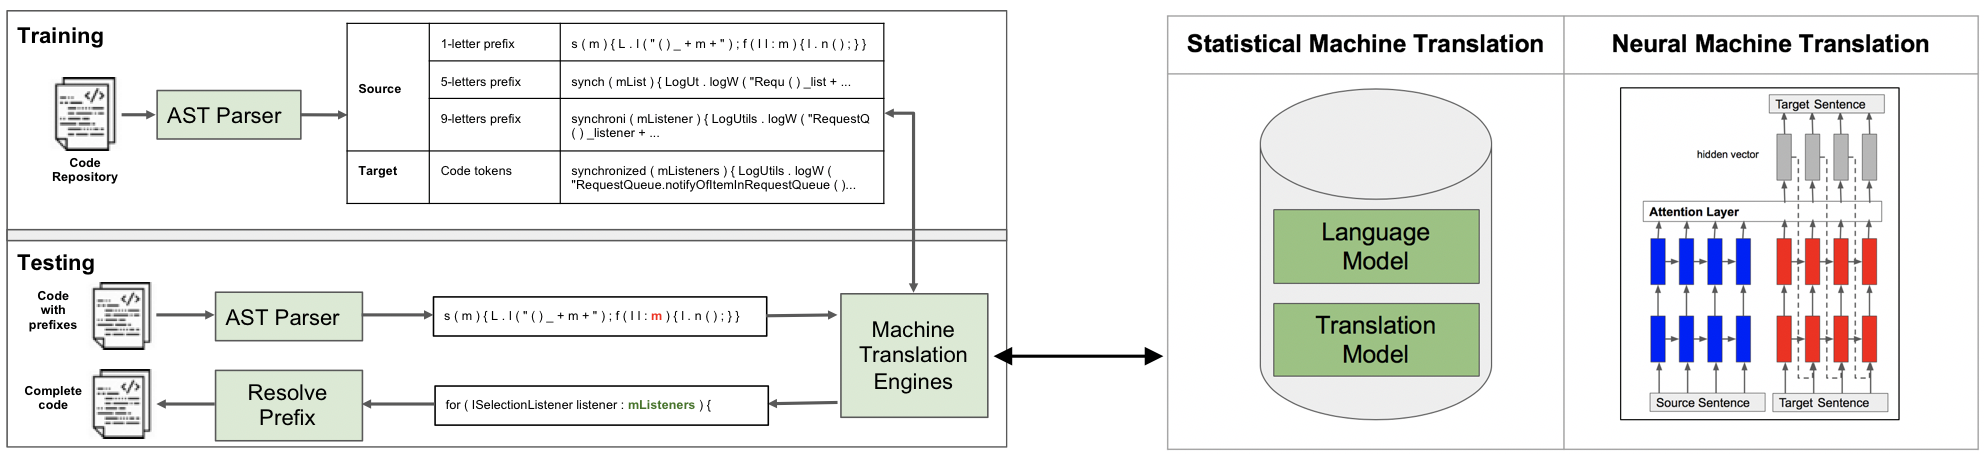
\includegraphics[width=\linewidth]
        {images/architecture.png}}
        \caption{PrefixMap Architecture Overview}
        \label{fig:mapping_expression} 
\end{figure*}
